\documentclass[12pt,twoside]{article}
%%%%%%%%%%%%%%%%%%%%%%%%%%%%%%%%%%%%%%%%%%%%%%%%%%%%%%%%%%%%%
% Meta informations:
\newcommand{\trauthor}{Weipeng He}
\newcommand{\trtype}{Seminar Paper} %{Seminararbeit} %{Proseminararbeit}
\newcommand{\trcourse}{Bio-inspired Artificial Intelligence}
\newcommand{\trtitle}{Self-replicating Robots : A review}
\newcommand{\trmatrikelnummer}{6411529}
\newcommand{\tremail}{2he@informatik.uni-hamburg.de}
\newcommand{\trarbeitsbereich}{Knowledge Technology, WTM}
\newcommand{\trdate}{\today}

%%%%%%%%%%%%%%%%%%%%%%%%%%%%%%%%%%%%%%%%%%%%%%%%%%%%%%%%%%%%%
% Languages:

% Falls die Ausarbeitung in Deutsch erfolgt:
% \usepackage[german]{babel}
% \usepackage[T1]{fontenc}
% \usepackage[latin1]{inputenc}
% \usepackage[latin9]{inputenc}	 				
% \selectlanguage{german}

% If the thesis is written in English:
\usepackage[english]{babel} 						
\selectlanguage{english}

%%%%%%%%%%%%%%%%%%%%%%%%%%%%%%%%%%%%%%%%%%%%%%%%%%%%%%%%%%%%%
% Bind packages:
\usepackage{acronym}                    % Acronyms
\usepackage{algorithmic}								% Algorithms and Pseudocode
\usepackage{algorithm}									% Algorithms and Pseudocode
\usepackage{amsfonts}                   % AMS Math Packet (Fonts)
\usepackage{amsmath}                    % AMS Math Packet
\usepackage{amssymb}                    % Additional mathematical symbols
\usepackage{amsthm}
\usepackage{booktabs}                   % Nicer tables
%\usepackage[font=small,labelfont=bf]{caption} % Numbered captions for figures
\usepackage{color}                      % Enables defining of colors via \definecolor
\definecolor{uhhRed}{RGB}{254,0,0}		  % Official Uni Hamburg Red
\definecolor{uhhGrey}{RGB}{122,122,120} % Official Uni Hamburg Grey
\usepackage{fancybox}                   % Gleichungen einrahmen
\usepackage{fancyhdr}										% Packet for nicer headers
%\usepackage{fancyheadings}             % Nicer numbering of headlines

%\usepackage[outer=3.35cm]{geometry} 	  % Type area (size, margins...) !!!Release version
%\usepackage[outer=2.5cm]{geometry} 		% Type area (size, margins...) !!!Print version
%\usepackage{geometry} 									% Type area (size, margins...) !!!Proofread version
\usepackage[outer=3.15cm]{geometry} 	  % Type area (size, margins...) !!!Draft version
\geometry{a4paper,body={5.8in,9in}}

\usepackage{graphicx}                   % Inclusion of graphics
%\usepackage{latexsym}                  % Special symbols
\usepackage{longtable}									% Allow tables over several parges
\usepackage{listings}                   % Nicer source code listings
\usepackage{multicol}										% Content of a table over several columns
\usepackage{multirow}										% Content of a table over several rows
\usepackage{rotating}										% Alows to rotate text and objects
\usepackage[hang]{subfigure}            % Allows to use multiple (partial) figures in a fig
%\usepackage[font=footnotesize,labelfont=rm]{subfig}	% Pictures in a floating environment
\usepackage{tabularx}										% Tables with fixed width but variable rows
\usepackage{url,xspace,boxedminipage}   % Accurate display of URLs

%%%%%%%%%%%%%%%%%%%%%%%%%%%%%%%%%%%%%%%%%%%%%%%%%%%%%%%%%%%%%
% Configurationen:

\hyphenation{whe-ther} 									% Manually use: "\-" in a word: Staats\-ver\-trag

%\lstloadlanguages{C}                   % Set the default language for listings
\DeclareGraphicsExtensions{.pdf,.svg,.jpg,.png,.eps} % first try pdf, then eps, png and jpg
\graphicspath{{./data/}} 								% Path to a folder where all pictures are located
\pagestyle{fancy} 											% Use nicer header and footer

% Redefine the environments for floating objects:
\setcounter{topnumber}{3}
\setcounter{bottomnumber}{2}
\setcounter{totalnumber}{4}
\renewcommand{\topfraction}{0.9} 			  %Standard: 0.7
\renewcommand{\bottomfraction}{0.5}		  %Standard: 0.3
\renewcommand{\textfraction}{0.1}		  	%Standard: 0.2
\renewcommand{\floatpagefraction}{0.8} 	%Standard: 0.5

% Tables with a nicer padding:
\renewcommand{\arraystretch}{1.2}

%%%%%%%%%%%%%%%%%%%%%%%%%%%%
% Additional 'theorem' and 'definition' blocks:
\theoremstyle{plain}
\newtheorem{theorem}{Theorem}[section]
%\newtheorem{theorem}{Satz}[section]		% Wenn in Deutsch geschrieben wird.
\newtheorem{axiom}{Axiom}[section] 	
%\newtheorem{axiom}{Fakt}[chapter]			% Wenn in Deutsch geschrieben wird.
%Usage:%\begin{axiom}[optional description]%Main part%\end{fakt}

\theoremstyle{definition}
\newtheorem{definition}{Definition}[section]

%Additional types of axioms:
\newtheorem{lemma}[axiom]{Lemma}
\newtheorem{observation}[axiom]{Observation}

%Additional types of definitions:
\theoremstyle{remark}
%\newtheorem{remark}[definition]{Bemerkung} % Wenn in Deutsch geschrieben wird.
\newtheorem{remark}[definition]{Remark} 

%%%%%%%%%%%%%%%%%%%%%%%%%%%%
% Provides TODOs within the margin:
\newcommand{\TODO}[1]{\marginpar{\emph{\small{{\bf TODO: } #1}}}}

%%%%%%%%%%%%%%%%%%%%%%%%%%%%
% Provides latin abbriviations:
\newcommand{\etal}{\textit{et al.}}
\newcommand{\etc}{\textit{etc.}}
\newcommand{\eg}{\textit{e.g.}}

%%%%%%%%%%%%%%%%%%%%%%%%%%%%
% Abbreviations and mathematical symbols
\newcommand{\modd}{\text{ mod }}
\newcommand{\RS}{\mathbb{R}}
\newcommand{\NS}{\mathbb{N}}
\newcommand{\ZS}{\mathbb{Z}}
\newcommand{\dnormal}{\mathit{N}}
\newcommand{\duniform}{\mathit{U}}

\newcommand{\erdos}{Erd\H{o}s}
\newcommand{\renyi}{-R\'{e}nyi}
%%%%%%%%%%%%%%%%%%%%%%%%%%%%%%%%%%%%%%%%%%%%%%%%%%%%%%%%%%%%%
% Document:
\begin{document}
\renewcommand{\headheight}{14.5pt}

\fancyhead{}
\fancyhead[LE]{ \slshape \trauthor}
\fancyhead[LO]{}
\fancyhead[RE]{}
\fancyhead[RO]{ \slshape \trtitle}

%%%%%%%%%%%%%%%%%%%%%%%%%%%%
% Cover Header:
\begin{titlepage}
	\begin{flushleft}
		Universit\"at Hamburg\\
		Department Informatik\\
		\trarbeitsbereich\\
	\end{flushleft}
	\vspace{3.5cm}
	\begin{center}
		\huge \trtitle\\
	\end{center}
	\vspace{3.5cm}
	\begin{center}
		\normalsize\trtype\\
		[0.2cm]
		\Large\trcourse\\
		[1.5cm]
		\Large \trauthor\\
		[0.2cm]
		\normalsize Matr.Nr. \trmatrikelnummer\\
		[0.2cm]
		\normalsize\tremail\\
		[1.5cm]
		\Large \trdate
	\end{center}
	\vfill
\end{titlepage}

	%backsite of cover sheet is empty!
\thispagestyle{empty}
\hspace{1cm}
\newpage

%%%%%%%%%%%%%%%%%%%%%%%%%%%%
% Abstract:

% Abstract gives a brief summary of the main points of a paper:
\section*{Abstract}
In the past few years, the field of self-replicating robotics has advanced from proof-of-concept systems to physical implementations. This technology of imitating living organisms has many important applications as well as Platonic appeal for scientist.

In this review paper, we discuss the recent studies on self-replicating robotics. We categorize those techniques to three different types: directed replication via fabrication, directed replication via module assembly, self-assembly of randomly agitated modules. These different approaches are evaluated. Each type has its advantage and limitation. The combination of multiple types is promising in future research.

% Lists:
\tableofcontents
\pagenumbering{arabic}
\clearpage

%%%%%%%%%%%%%%%%%%%%%%%%%%%%
% Content:

% the actual content, usually separated over a number of sections
% each section is assigned a label, in order to be able to put a
% crossreference to it

\section{Introduction}
\label{sec:intro}

\subsection{Self-replication and self-reproduction}
Self-replication is the process of a machine by which an identical functional copy of itself is created automatically. The concept of self-replication derives from the reproduction process of living organism. Thus, the study of self-replicating machines is intriguing because it embodies the romantic idea of making artificial machines which can imitate the real lives.

The reproduction process in nature, however, does not make the identical copy of the parent(s). That is to say, errors, which might be good or not, happen in this process.  So is it with the self-reproduction of machines, which is also a topic for computer scientists. The self-reproduction is the process of a machine autonomously creating an approximate copy of itself.

However, according to The Second Law of Thermodynamics and Shannon's theorem about information, it is impossible to copy information without any loss. Therefore, we consider the error of replication can be within specified tolerances so that the replica still
works as well as the original \cite{jones_reprap_2011}.

\subsection{Self-replicating robots}
Research in self-replication was introduced by John von Neumann\cite{von_neumann_theory_1962} more than 60 years ago. Yet it was not until the last decade that researchers implemented physical self-replicating robots\cite{suthakorn_autonomous_2003}. 

The applications for self-replication also break through from theoretical work to practical projects. Originally proposed in a NASA project of advanced automation for space missions \cite{freitas_report_1981}, the applications of self-replicating robots for space exploration and development have been promoted by recent achievements of physically realized self-replicating robots\cite{chirikjian_self-replicating_2002}. The exponential growth of self-replicating robots can minimize the launch payload and free human from working on-site.

Although many excellent works in theoretical self-replicating machines, especially in cellular automata, are studied by scientist, in this paper we only focus on those designs that have already been physically implemented or at least are apparently easy to realize.

\subsection{Categorization}
Lee \etal\cite{lee_robotic_2008} classified the recent work on self-replicating robots into four categories. We adopted three of them, which will be discussed in this review paper :

  \emph{Directed replication via fabrication}: Using rapid prototyping technology, a 3-D printer make a replica of itself out of raw material.
  
  \emph{Directed replication via module assembly}: A modular robot executes a directed sequence of movement to assemble prepared spare modules to a replica robot.
  
  \emph{Self-assembly of randomly agitated modules}: Modules are kept moving randomly in a environment with external work source, and then assemble to functional parts through a stochastic process.

We exclude the category, self-reconfigurable modular robots, for the reason that it is not close related to the topic of self-replication. Although some technology of self-reconfigurable modular robots are basics for self-replicable modular robots, they are not necessarily able to replicate.

\subsection{Attributes for self-replicating robots}
\label{sec:attri}
To evaluate the quality of a self-replicating robots, we discuss the following attributes, which are closely related to the implementation and application for self-replicating robots:

\emph{Input complexity}: For the replication process, there must be physical input, which is the raw materials. The raw materials can be spare robot modules, plastic, metal or substance from nature. We expect the robots can take materials of lower complexity as the input, so that the robots have higher adaptation in the environment. However, using nature substance as raw material is still an ideal goal for the researchers. So far, we consider those self-replicating robots that use plastic and metal as raw materials are better than those use complex spare robot modules.
  
\emph{Working environment}: Robots work in different environments. Some are artificially set up, while other are not. According to it artificial level, the working environment can be categorized in three level\cite{lee_robotic_2007} : structured environment, semi-structured environment and unstructured environment. In structured environment, objects are placed in exact precise location with predefined order. In semi-structured or partially structured environment, objects are placed in exact location with small error and random order. An unstructured environment is without any structure resulting from initial human intervention.
  
\emph{Autonomy of design}: While the replication process of robots can be totally designed by developers, it is also possible to use evolution algorithm for the design with less predefined knowledge. The evolution ability will be quite essential in future designs as both the structures of the robots and the environment will be more complex, which make it more difficult for researchers to find out a proper procedure for replication.

% \emph{Degree of complexity}: Both Lee \etal\cite{lee_robotic_2008} and Adams \etal\cite{adams_universal_2009} proposed methods to measure the degree of complexity of the replication process. \TODO{}
% 
% \subsection{Difficulties in self-replicating robots}
% \TODO{} 

\subsection{Structure of this paper}
In this paper, I review the three categories of self-replicating robots. Each category is represented by one or two recent achievements. 

In section \ref{sec:fabri}, I will talk about machines of directed replication via fabrication and give the example of RepRap. In section \ref{sec:module}, I will introduce robots of directed replication via module assembly. One of the example, Molecubes, and its evolutionary design will be shown. In section \ref{sec:random}, the third type, self-assembly of randomly agitated modules, and two examples will be talked about. In section \ref{sec:discuss}, I will discuss and compare the three types of self-replicating robots.

\section{Directed replication via fabrication}
\label{sec:fabri}

As mentioned before, we can directly use rapid prototypers to manufacture the copy of the machines themselves. Examples are RepRap machine\cite{jones_reprap_2011}, cyclic fabrication system(CFS)\cite{moses_towards_2009} and Fab@Home machine\cite{malone_fabhome:_2007}.

\subsection{Rapid prototypers}
Rapid prototypers or 3D printers are machines that can rapidly fabricate objects on demand from computer-generated design specifications(such as CAD models)\cite{lipson_homemade_2005}. These prototypers usually take thermoplastic polymers as the raw materials. Either addition techniques (aggregation of melted plastics) or subtraction techniques (sculpture from a piece of raw plastics) is used to get the specified shape.

In the past 30 years, rapid prototyping have been favored by the manufacturing industry, as such technologies can enormously shorten the design period of new products. Recently, scientists made it possible to use prototypers in laboratories or at home.

\subsection{RepRap}
RepRap is an open-source project for self-replicating rapid prototyping machines\cite{jones_reprap_2011} (see figure \ref{fig:reprap}). The machine adopted fused-filament
fabrication as the core technique to make product from thermoplastic polymers.
RepRap is one of the state-of-the-art self-replicating fabricators, as it is capable to create most of its own part, while the rest part are components which are relatively easy to make or to purchase from the market.

\begin{figure}[b]
	 \centerline{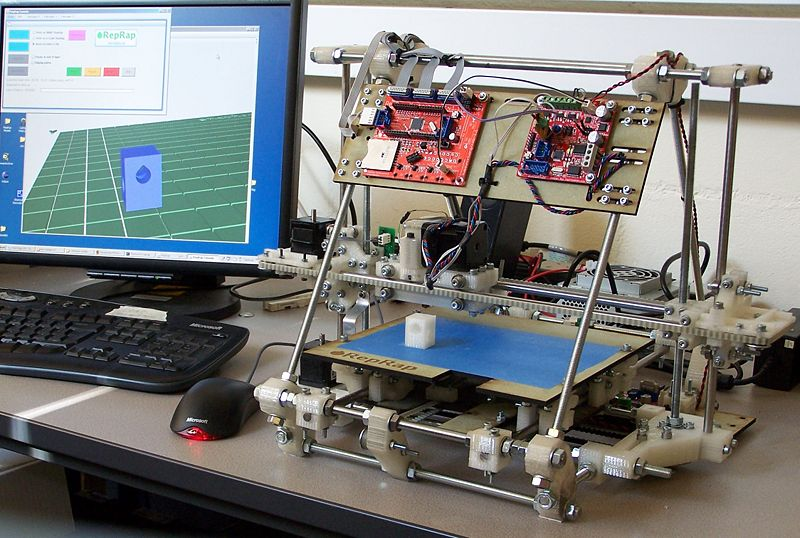
\includegraphics[width=0.7\textwidth]{mendel}}
	 {\caption{RepRap Version II ``Mendel'' (from \cite{jones_reprap_2011})}
	 \label{fig:reprap}}
\end{figure}

Different from other rapid prototyper, RepRap adapted several features to make the machine itself simple enough to self-manufacture. RepRap machine are designed to be small and light weight. Most of building materials are polylactic acid(PLA), which is hard, resistant to contraction problems on cooling and has medium melding point. RepRap also avoids complicated components, such as laser and inkjet print head, in its design.

As reported by the authors, the second version of RepRap machine can produce up to 57\% of its own part. The number of RepRap machines are estimated to be increased from 4 to 4500 via self-replication in two and half years(from 2008 to 2011). The success in growth of number of derived copies also indicates that the child machine are made within the tolerance of error.

While the machine is capable to create its consisting components, it cannot autonomously assemble the produced parts. As a matter of fact, the machine are assembled with manual assistance. Of course, the autonomous assembly, which is another field of study, can be applied.

\section{Directed replication via module assembly}
\label{sec:module}
Directed replication via module assembly is an approach to self-replication from another aspect. Other than focusing on fabrication, studies on these types of robots focus on autonomous assembly of simple functional modules to a more versatile structure. Physically realized self-replicating modular robots include Suthakorn \etal\cite{suthakorn_autonomous_2003}, Zykov \textit{et al}\cite{zykov_self-reproducing_2005}, Kaloutsakis and Chirikjian\cite{kaloutsakis_stochastic_2011}.

\subsection{Modular self-reconfigurable robots}
Modular self-reconfigurable robots are those system that are able to deliberately
change their own shape by rearranging the connectivity of their parts in order to
adapt to new circumstances, perform new tasks, or recover from damage\cite{yim_modular_2007}. The reconfiguration can be manual or automatic executed by disconnecting and reconnecting the modules in different arrangements.

Modular self-reconfigurable robots consist of simpler units and larger number of units are suitable for self-replication, as it is easy to program such robots to assemble spare modules into copies. 

\subsection{Molecubes}
Researchers from Cornell University (Zykov \etal) implemented Molecubes, which physically demonstrates the ability of self-replication\cite{zykov_self-reproducing_2005}\cite{zykov_evolved_2007}. 

\begin{figure}[t]
	 \centerline{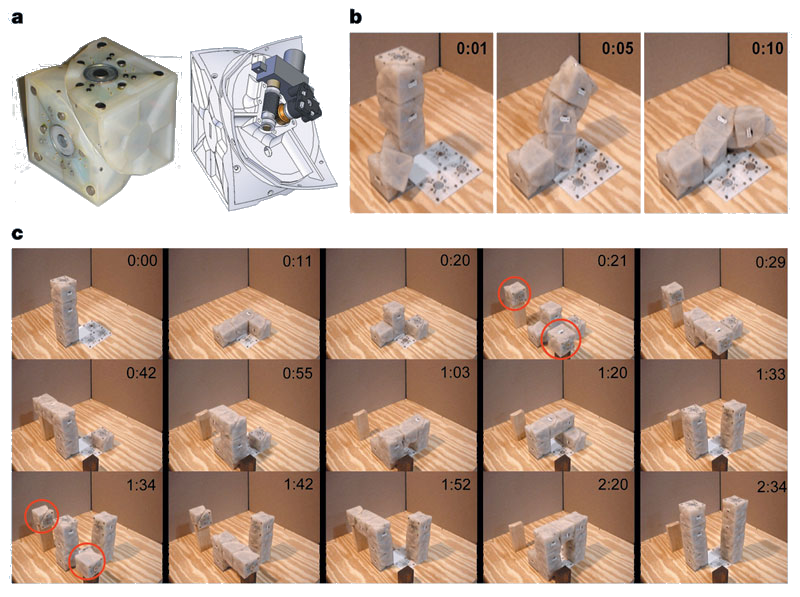
\includegraphics[width=\textwidth]{molecubes}}
	 {\caption{Molecubes (from \cite{zykov_self-reproducing_2005})}
	 \label{fig:mole}}
\end{figure}

The robot consists of modules of 10cm cube, of which the two halves can rotate about the long diagnose(see figure \ref{fig:mole}a). Therefore, each module has one degree of freedom(DOF). The six surfaces of the module are equipped with switchable electromagnet, which can be the state of ``north'', ``south'' and ``off''. Thus, the cubes are able to attract or repel the neighbor cubes. Power and information can also be transmitted to neighbor cubes via adjacent surfaces, that are attached. Multiple modules can be assembled to form a chain-like or other shapes. And, the assembled modules can perform more complicated moves(see figure \ref{fig:mole}b). 

The self-replication process is performed in a highly structured environment with some extent of human assistance. The Molecubes are placed on a desk with regular grids. Some of the grids provide the Molecubes with attaching points and 12V power supply. There are also some special grids called ``feeding'' location. At those location, spare modules are replenished. That is the only human intervention during the whole reproduction process.

The replication procedure, namely the sequence of movement, is manually designed. Physical experiments in self-replication of 3-module and 4-module robots were carried out. Figure \ref{fig:mole}c shows the self-replication process of the 4-module robot. The process spans out two and half minutes. At first, the original robot is provided. It moves and places its own module to specific location. Then, it picks up spare module from ``feeding'' locations, which is circled in red in the figure. At the end, the identical replica of the 4-module robot is assembled. Their experiments also show that the replica also successfully replicates itself. They also showed their design of replicating sequences for 2n-module ($n > 1$) robots. 

\subsection{Evolved design}
Rather than design the robots shape and replicating sequence manually, Zykov \etal also proposed an evolved design method for 2-D Molecubes in a simulating environment\cite{zykov_evolved_2007}.

The 2-D Molecubes are similar to 3-D Molecubes but the model is 2 dimensional and the modules are of two different types. The two types of the modules are swiveling blocks with permanent magnets and non-swiveling blocks with switchable electromagnet (an ``end-effector''). Like its 3-D version, the swiveling blocks can rotate about it diagnose. An ``end-effector'' are able to take the initiative to attach to another cube. Figure \ref{fig:2dmole}a shows an example of 2-D Molecubes and demonstrate how the swiveling blocks work.

\begin{figure}[t]
	 \centerline{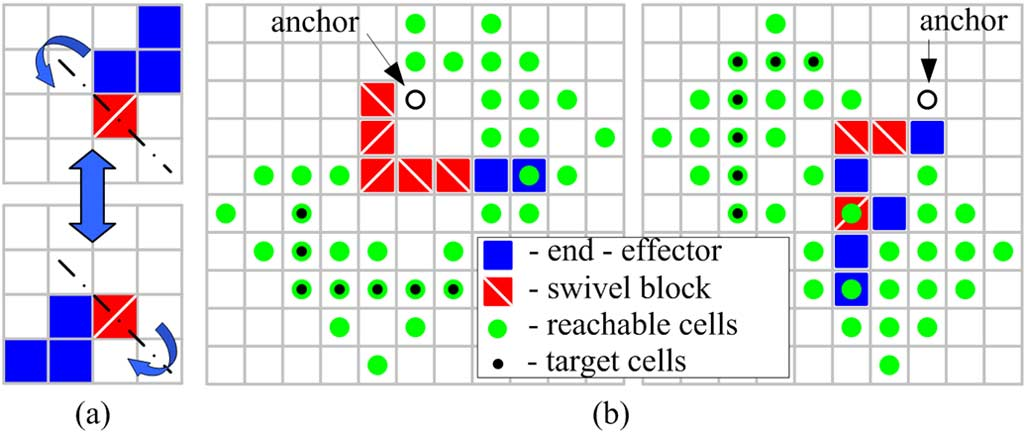
\includegraphics[width=.7\textwidth]{zykov-271}}
	 {\caption{2-D Molecubes (a) Swiveling module can swivel above the diagnose (b) Demonstration of reachable area (from \cite{zykov_evolved_2007})}
	 \label{fig:2dmole}}
\end{figure}

\begin{figure}[t]
	 \centerline{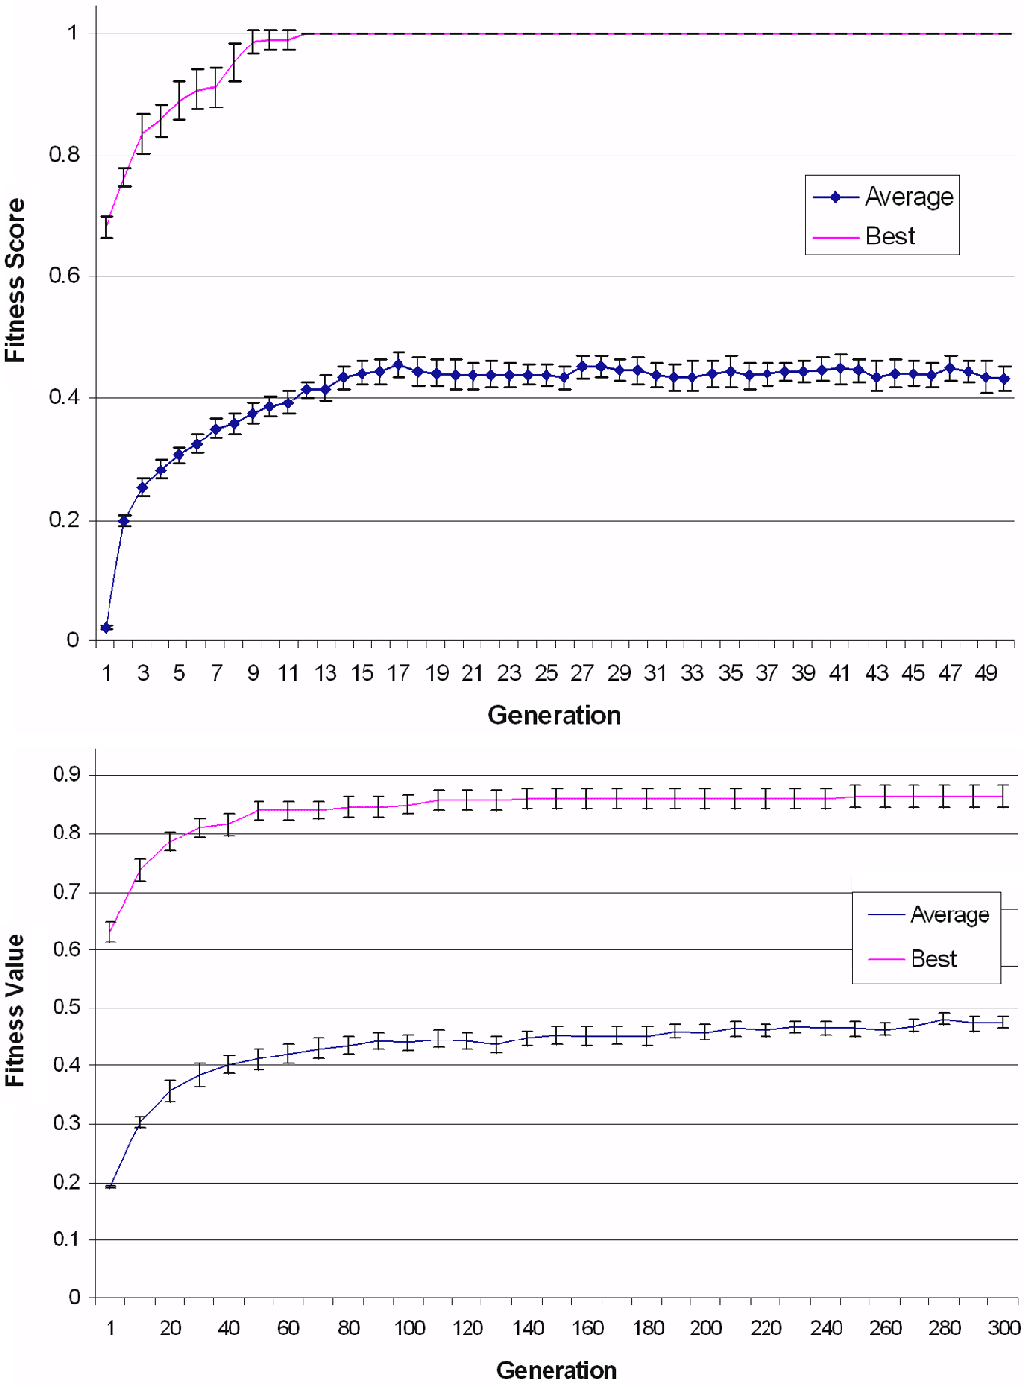
\includegraphics[width=.6\textwidth]{zykov-280}}
	 {\caption{Fitness value changes over generations. (top) Stage of morphology search. (bottom) Stage of controller search. (from \cite{zykov_evolved_2007})}
	 \label{fig:fitness}}
\end{figure}

The evolution algorithm consists of two stages. The first stage is to evolve the morphology of the machine, and the second stage is to evolve the control sequence of the robot.

\begin{figure}[t]
	 \centerline{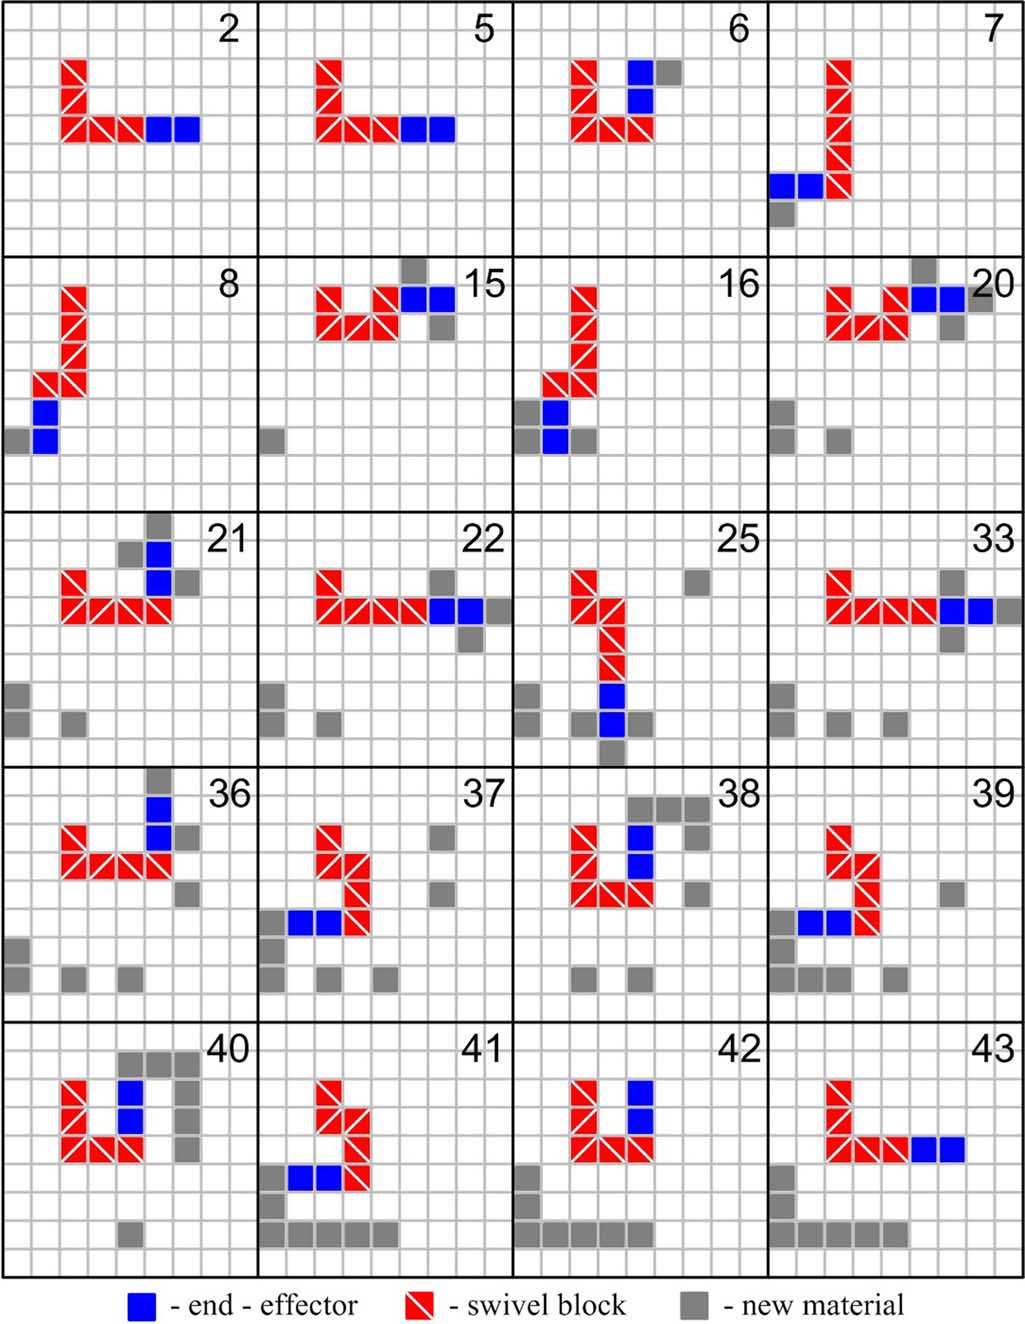
\includegraphics[width=.6\textwidth]{zykov-279}}
	 {\caption{Replication process of the L-shape robot. Some intermediate states is not shown.(from \cite{zykov_evolved_2007})}
	 \label{fig:l-repproc}}
\end{figure}

During the morphology evolving stage, a ``good'' shape for self-replication is automatically found. As there are millions of combinations and layouts of the modules, the varied morphology of the robot can result in different capability of reaching to the surrounding area. It is necessary for the robot to reach an area that contains the detached copy of itself and the dispenser(``feeding'') locations. Figure \ref{fig:2dmole}a shows the reachable area of an L-shape robot and an F-shape robot. In this stage, the fitness function is defined by coverage of the goal location :
\[ fitness = \frac{|reachableArea \cap goalArea|}{|goalArea|} \] where the $reachableArea$ is the area of those cells adjacent to at least one ``end-effector'' in any state and the $goalArea$ is the area of the copy. A variable-length gnome is defined to represent a morphology of the machine. One of the results of the evolutionary search is the L-shape robot in Figure \ref{fig:2dmole}a. The fitness value during the evolution process is shown in Figure \ref{fig:fitness}(top).

In the second stage, the robot evolves a sequence of moves to making a replica of itself. The fitness function is given as below: 
\[ fitness = 0.8p + 0.2 \frac{c - s + 1}{c} - 0.03 e \] 
where $p$ is the weighted fraction of the goal location covered; $c$ is number of blocks inside the model; $s$ is number of dispensers and $e$ is number of excess blocks beyond those needed. The gnome for the controlling sequence is a string of three different types of move, which are (1) trying to swivel a swiveling block (2) attach a new block from its end-effector (3) detach a copy block from its end-effector. Using evolutionary search, possible replicating sequences are found. Same as the first stage, the fitness value is shown in  Figure \ref{fig:fitness}(bottom). Figure \ref{fig:l-repproc} shows one of the replication process of the L-shape robot.

\section{Self-assembly of randomly agitated modules}
\label{sec:random}

Self-assembly of randomly agitated modules is another type of self-replication. Although the robots are also assembled from modules, it is quite different from directed replication via module assembly, as it does not apply a fixed sequence of ``pick-and-place'' but the whole assembly process are randomly performed.

Note that self-assembly does not imply self-replication. In this section, we refer the term ``Self-assembly of randomly agitated modules'' to those robots that can be assembled to have the same structure with the template's. 

The replication process of DNA, which is well studied by biology scientists, gives an inspiration for designing self-replicating robots. The building blocks of DNA, nucleotides, are randomly distributed in the cell environment. While they are moving randomly, they have the opportunity to be acquired by the template DNA. With the help of DNA polymerase, the DNA can using the acquired nucleotides to replicate itself. The biology system also has a technique to proofread the replicated DNA in order to assure the precision of replication\cite{alberts_molecular_2002}. Such intricate process can be adapted to robots systems.

The earliest design of this kind of self-replicating robots can be dated back to 1957\cite{penrose_self-reproducing_1957}. Recently, Griffith \etal \cite{griffith_self-replication_2005} and Matsumoto \etal \cite{matsumoto_passive_2009} both realized self-replicating robots of the same type.

\subsection{Girffith's design}
Using electromechanical modules randomly floating on an air table, Griffith \etal realized a self-replicating robot which can imitate the DNA replication process\cite{griffith_growing_2004}\cite{griffith_self-replication_2005}. They conducted experiments on self-replication of 5-bit strings, which successfully showed that the robot can replicate autonomously and attain an exponential growth while the supplying modules are sufficient.

\begin{figure}[t]
	 \centerline{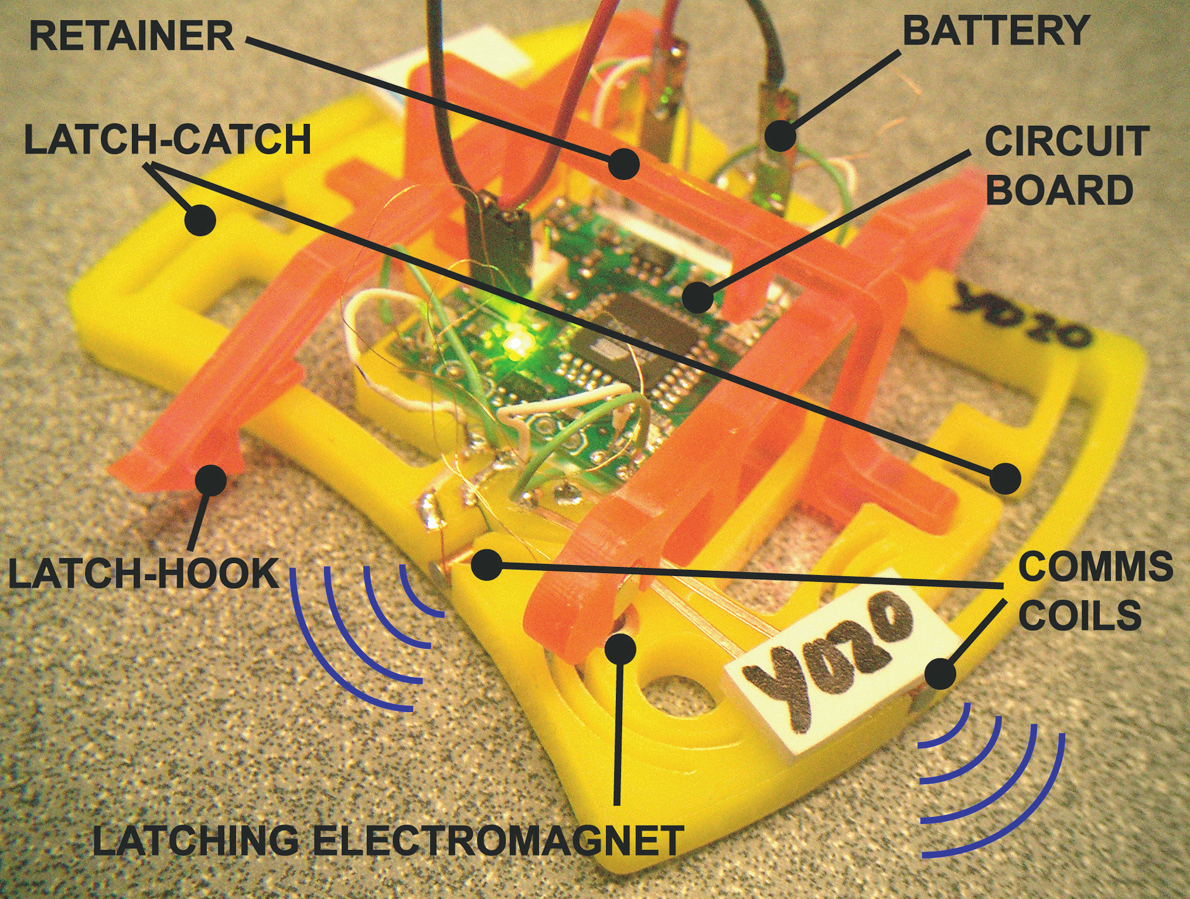
\includegraphics[width=.4\textwidth]{griffith-000}}
	 {\caption{The basic module of the self-replicating robot. The module can communicate with and attach to other modules nearby. (from \cite{griffith_growing_2004})}
	 \label{fig:gri-unit}}
\end{figure}

\begin{figure}[t]
	 \centerline{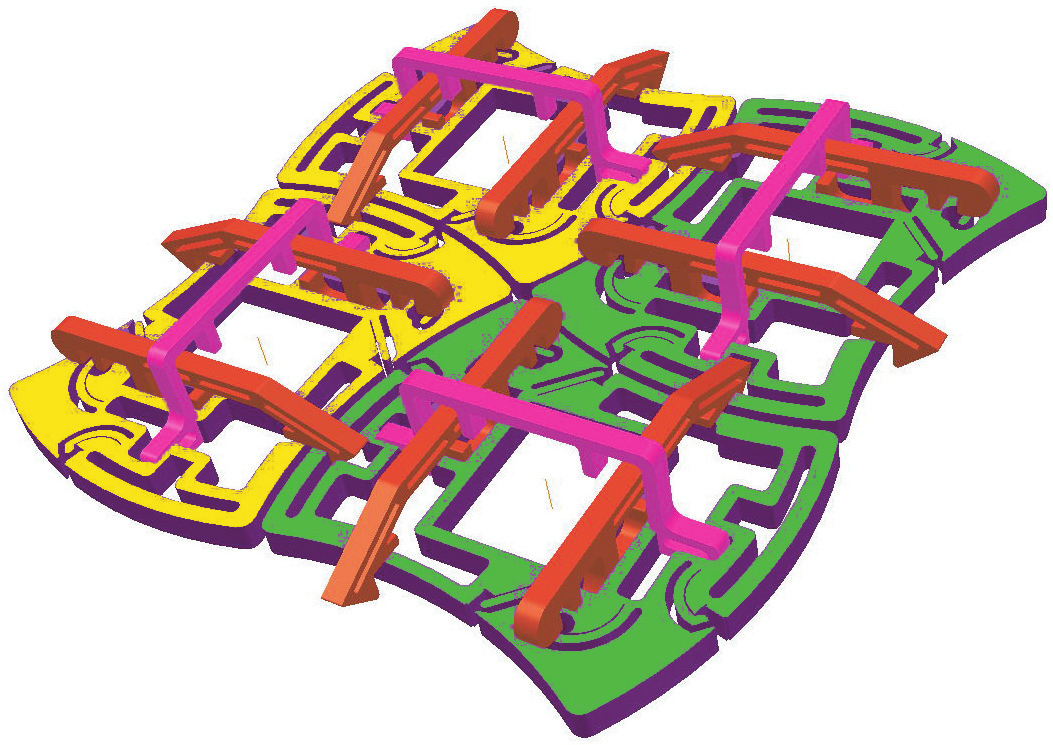
\includegraphics[width=.4\textwidth]{griffith-001}}
	 {\caption{Four modules are successfully assembled in a square lattice (from \cite{griffith_growing_2004})}
	 \label{fig:gri-sqr}}
\end{figure}

The basic module for this robot is a square-like shaped plastic plate equipped with circuit board, latches and communicating coils (See figure \ref{fig:gri-unit}). The two pairs of opposite edges are convex and concave respectively. The design of this shape makes them possible to tessellate in a 2-D space. It also reduces the complexity for assembling, as it requires the attaching modules place in a specific orientation. Furthermore, their mechanical experiments have shown that this shape increases the likelihood of successful binding upon collision. Figure \ref{fig:gri-sqr} shows that four modules are successfully assembled in a square lattice. 

There are two types of modules, green and yellow, which are identical in shape. It's the micro-controller on the circuit board that identifies the type of the module. The communicating coils allows the modules to communicate via wireless network with other modules within the distance of 10mm. Thus, neighbor modules mutually can know the type of others. 

Each module has two latch-hooks and two latch-catches. The latch-hooks are controlled by electromagnets, which are directly connected to the micro-controller. Therefore, the module can change its state with adjacent modules via turning on and off the hook. Comparing to pure electromagnet latching, this design is less power consuming, and more suitable for the floating module. 

The latching behavior of each module is controlled by a 7-state, finite-state machine in the micro-controller. The finite-state machine also carries out error-checking mechanism, which is essential for complex system.

At the beginning of their experiment, a template 5-bit string (5 linearly connected modules) together with supplying modules are put on an air table. As the modules move randomly on the table, they are acquired by the template string by chances. Self-similarity of the acquired module is checked for the modules to decide whether to keep or release. After finishing replication, the copy is released and becomes another template. Thus, the number of the specific template strings grows exponentially as long as the spare modules are sufficient.

\begin{figure}[t]
	 \centerline{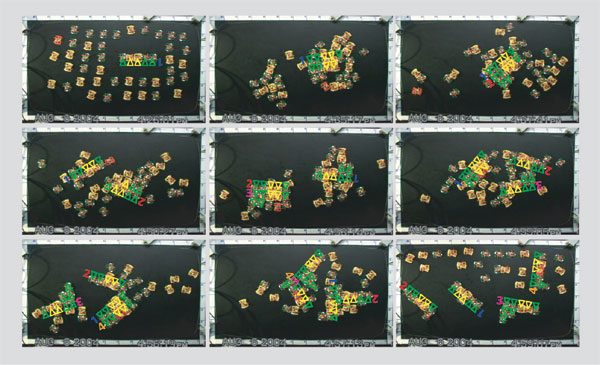
\includegraphics[width=1\textwidth]{griffith-1}}
	 {\caption{ Snapshots taken during the self-replication of a 5-bit string. (from \cite{griffith_self-replication_2005})}
	 \label{fig:gri-proc}}
\end{figure}

\begin{figure}[t]
	 \centerline{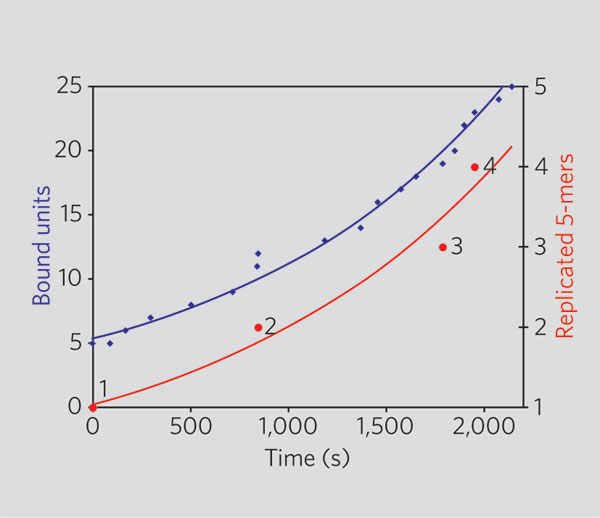
\includegraphics[width=.4\textwidth]{griffith}}
	 {\caption{ Replication kinetics for bound units (blue) and replicated strings (red) as a function of time (from \cite{griffith_self-replication_2005})}
	 \label{fig:gri-expo}}
\end{figure}

Figure \ref{fig:gri-proc} shows snapshots taken during the experiment. In frame 1, the initial 5-bit string (number 1, green, green, yellow, yellow, green) and several spare modules are placed on the table. In frame 2, spare modules are attached to the template string. From frame 3 to 9, 3 strings (number 2, 3, 4) are replicated according to the initial one. Figure \ref{fig:gri-expo} shows the number of bound units and replicated strings both increase exponentially through time. Strings are numbered as in Figure \ref{fig:gri-proc}.

Additionally, self-replication of other shape of robots (not only 1-D, but also 2-D patterns) is implemented too, using the same system.

\subsection{Matsumoto's design}
Matsumoto \etal proposed another self-replicating robot using randomly agitated modules\cite{matsumoto_passive_2009}. Comparing to Griffith's design, the module in their design is more simple in structure and the assembly is done in 3-D environment.

There are 3 types of basic modules (white, black and red). Figure \ref{fig:matsu-mod} shows their structure. The cubic unit has mortise and tenon on top and bottom surfaces. Modules of the same type have the complementary structure of mortise and tenon, while modules of different types do not. Thus, the selectivity of matching types is acquired. The hot-melt adhesive on the side surfaces and the solder on the top and bottom surfaces, provides the unit with two kinds of bonds, which correspond to the phosphodiester bond and the hydrogen bond in DNA. The hot-melt adhesive (melting point 78 $^\circ$C) make the chain of the units in one gene stick together. While, the solder (melting point 48 $^\circ$C) is responsible for binding of the matching modules.

Figure \ref{fig:matsu-env} shows the environment for experiment. The modules are floating in the solution during the replication process. The solution is chosen to be heated and stirred during different phase of the process. The phase changes from assembly mode to connection mode, and then division mode. The initial gene is replicated via repetition of the mode changing. Illustration of the replication process is in figure \ref{fig:matsu-modes}. 

Their experiments show successful autonomous self-replication of both 1-D genes and 2-D genes. Figure \ref{fig:matsu-res} shows the result of replication.

\begin{figure}[t]
	 \centerline{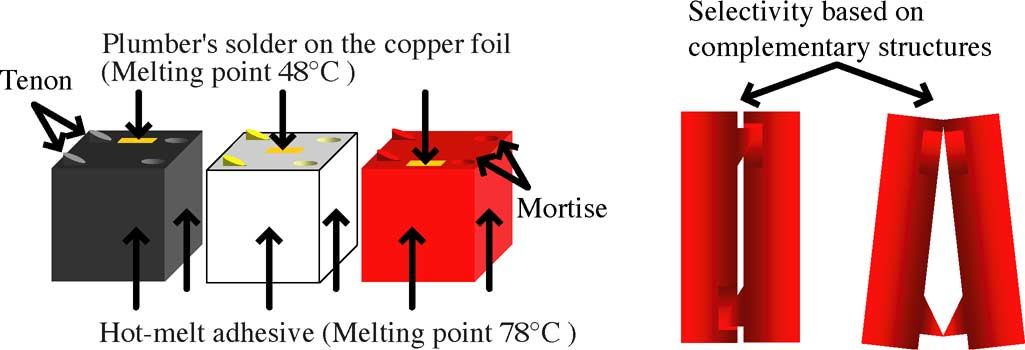
\includegraphics[width=.7\textwidth]{matsu-001}}
	 {\caption{Design of the basic module. (from \cite{matsumoto_passive_2009})}
	 \label{fig:matsu-mod}}
\end{figure}

\begin{figure}[h]
	 \centerline{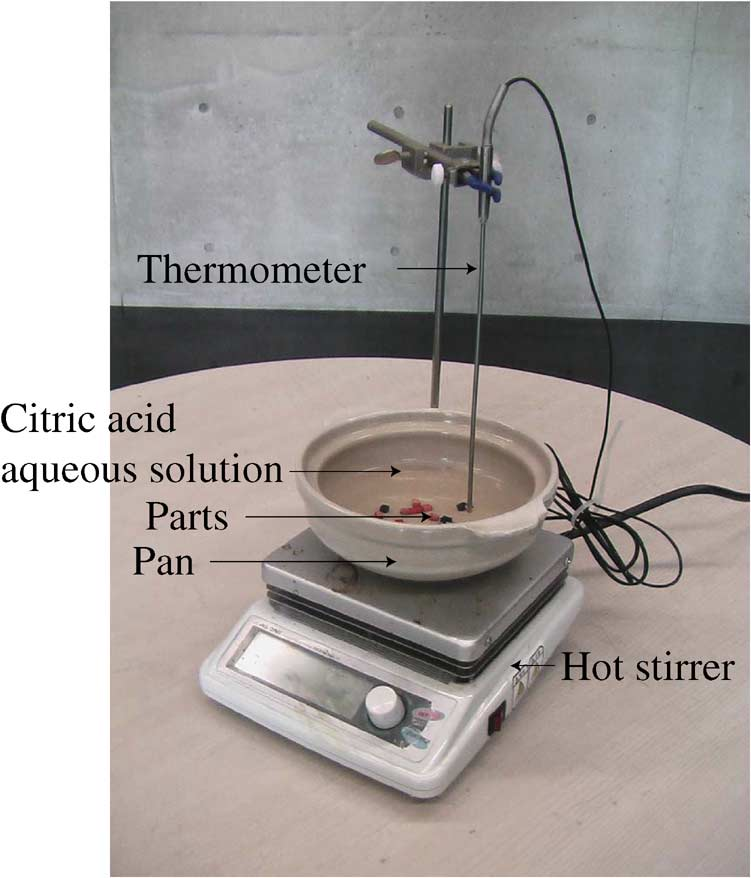
\includegraphics[width=.55\textwidth]{matsu-003}}
	 {\caption{The environment for experiment. (from \cite{matsumoto_passive_2009})}
	 \label{fig:matsu-env}}
\end{figure}

\begin{figure}[h]
	 \centerline{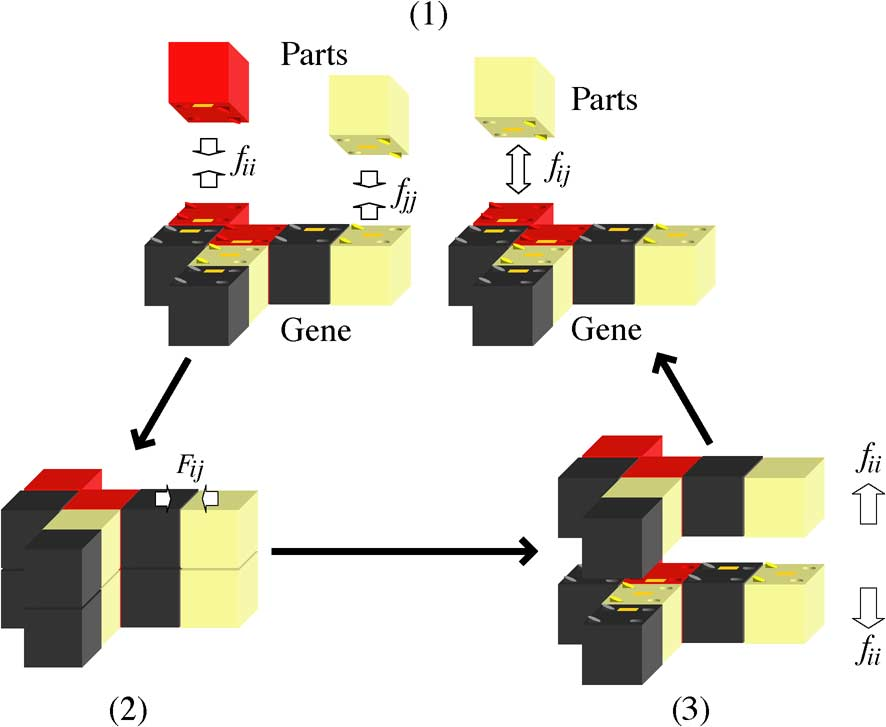
\includegraphics[width=.5\textwidth]{matsu-000}}
	 {\caption{The process of self-replication (from \cite{matsumoto_passive_2009})}
	 \label{fig:matsu-modes}}
\end{figure}

\begin{figure}[h]
	 \centerline{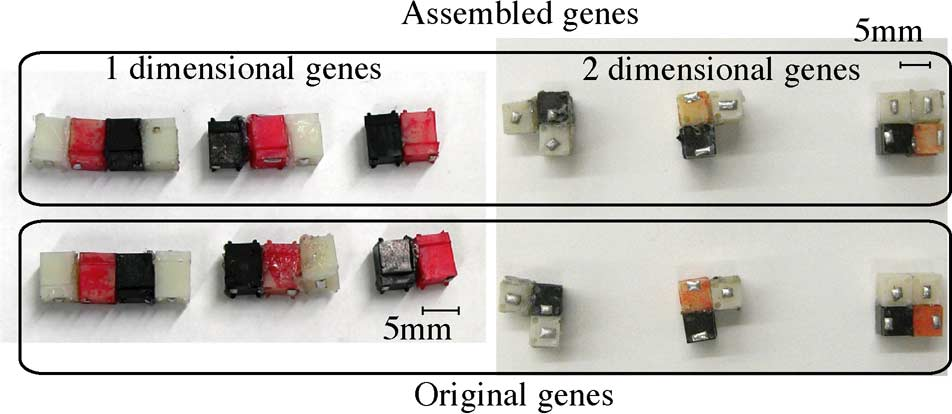
\includegraphics[width=.7\textwidth]{matsu-019}}
	 {\caption{Result of self-replication (from \cite{matsumoto_passive_2009})}
	 \label{fig:matsu-res}}
\end{figure}

\section{Discussion}
\label{sec:discuss}

In previous sections, we have described the theory and examples of three types of self-replicating robots, namely directed replication via fabrication, directed replication via module assembly and self-assembly of randomly agitated modules. Each type has realized physical self-replication from different approaches. In this section, we discuss their features according to the attributes we described in section \ref{sec:attri}.

Recent achievements of directed replication via fabrication (take RepRap as the example) has shown the ability of taking considerably low-complexity materials as input. Although these fabricating systems are still not able to fully construct themselves, they are essential prototypes for making self-replicating robots that take raw materials from environment. The limitation is that their working environment is largely dependent on human intervention. They require human to assemble their parts together. It is possible to adapt self-assembly function to their design. However, the addition of functional parts will result in making the machine itself more complex and hard to fabricate. The whole replication process is designed manually.

The robots of directed replication via module assembly consist of building blocks of high complexity. The robots are more versatile, but the cost of making the additional modules is high. As for the example robot (Molecubes), the robot works in a structured environment, with all additional modules placed in specific locations. This type of self-replicating robots successfully applies evolutionary computation for designing the morphology and control sequences. This application makes it possible to design more complex systems.

The third type, self-assembly of randomly agitated modules, has robot modules of medium complexity. The basic modules are possible to mass produce with low cost. The robots work in unstructured environments.

A short evaluation of the three categories is shown in table \ref{tab:eval}.

\begin{table}[ht]
  \centering
  \caption{This table shows some data}
  \label{tab:eval}
  \begin{tabular}{|p{4.3cm}|p{2cm}|p{4cm}|p{2.9cm}|}
    \hline 
    ~ & Input complexity & Working environment & Autonomy of Design \\
    \hline \hline
    directed replication via fabrication & Low & Dependent to human intervention & Manual \\
    \hline
    directed replication via module assembly & High & Structured environment & Evolved design \\
    \hline
    self-assembly of randomly agitated modules & Medium & Unstructured environment & Manual \\
    \hline
  \end{tabular}
\end{table}

Extending from John von Neumann's theory on self-replicating automata, scientists have achieved powerful, practical results in self-replicating robotics. Especially, various physically realized self-replicating robots demonstrate the ability of machines to imitate nature organisms from different aspects. In future researches, the combination of the three types of self-replicating robots is possible, in order to attain lowest input complexity and maximum functionality of the system.

%%%%%%%%%%%%%%%%%%%%%%%%%%%%%%%%%%%%%%
% hier werden - zum Ende des Textes - die bibliographischen Referenzen
% eingebunden
%
% Insbesondere stehen die eigentlichen Informationen in der Datei
% ``bib.bib''
%

\addcontentsline{toc}{section}{References}% Add to the TOC
\bibliography{bib}
\bibliographystyle{plain}

\end{document}
